\chapter{Sprint 3 – POS Interface \& Invoicing}

\section{Introduction}

The third sprint focused on developing the core cashier interface and implementing the complete invoicing system. While Sprint 2 established the administrative foundation for user and product management, Sprint 3 addressed the primary user-facing functionality: the point-of-sale interface that cashiers use for daily operations and the comprehensive invoicing system that completes transactions.

This sprint was crucial for delivering the core business value of the POS system, as it enables cashiers to efficiently process sales, manage customer transactions, and generate proper invoices for all purchases.

\section{Sprint 3 Backlog}

\begin{table}[H]
\centering
\begin{tabular}{|c|p{10cm}|c|}
\hline
\textbf{Task ID} & \textbf{Task Description} & \textbf{Status} \\
\hline
S3-T1 & Create POS cashier interface & Completed \\
S3-T2 & Build product browsing system & Completed \\
S3-T3 & Add shopping cart functionality & Completed \\
S3-T4 & Implement payment processing & Completed \\
S3-T5 & Create invoice generation & Completed \\
S3-T6 & Add QR code to invoices & Completed \\
S3-T7 & Update stock after sales & Completed \\
S3-T8 & Test POS functions & Completed \\
\hline
\end{tabular}
\caption{Sprint 3 – Backlog and Implementation Plan}
\label{tab:sprint3-backlog}
\end{table}

\section{Functional Specification}

The POS interface was designed to provide a streamlined experience for cashiers to process sales efficiently. The system includes:

\begin{itemize}
  \item \textbf{Product Display Grid:} Visual product catalog with images, names, and prices
  \item \textbf{Cart Management:} Real-time cart updates with quantity controls and total calculation
  \item \textbf{Payment Processing:} Multiple payment method support (cash, card, digital wallet)
  \item \textbf{Invoice Generation:} Automatic PDF creation with QR codes and transaction details
  \item \textbf{Stock Management:} Real-time inventory updates after successful transactions
  \item \textbf{Transaction Logging:} Complete audit trail for all sales activities
\end{itemize}

The interface was optimized for speed and ease of use during busy periods while maintaining accuracy and reliability.

\section{Use Case Diagram}

\begin{figure}[H]
  \centering
  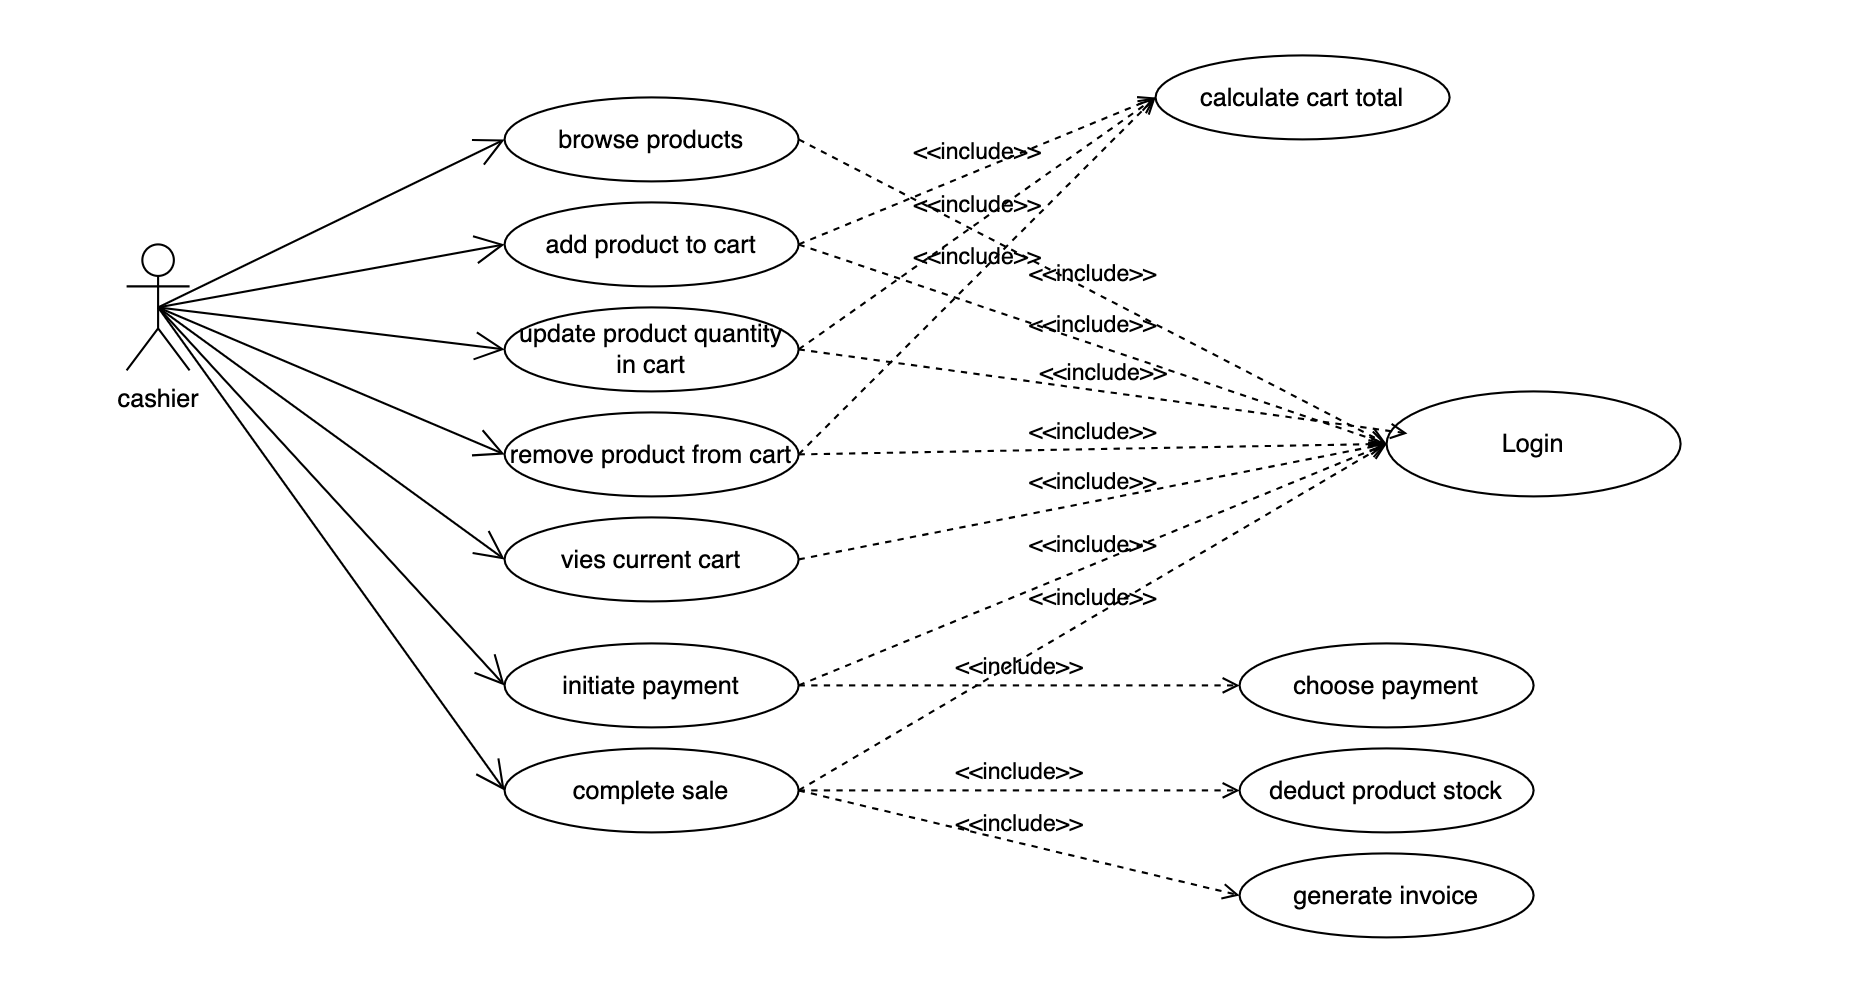
\includegraphics[width=0.9\textwidth]{figures/images/sprint3usecase.png}
  \caption{Sprint 3 – POS Interface and Invoicing Use Case Diagram}
  \label{fig:sprint3-usecase}
\end{figure}

\section{POS Interface Implementation}

\subsection*{Product Grid and Navigation}

The product display system features:
\begin{itemize}
  \item Responsive grid layout showing all available products
  \item Product cards with high-quality images, names, and current prices
  \item Category-based filtering for quick product location
  \item Search functionality for rapid product lookup
  \item Stock level indicators to prevent overselling
\end{itemize}

\subsection*{Shopping Cart Functionality}

The cart system provides:
\begin{itemize}
  \item One-click product addition with default quantity
  \item Quantity adjustment controls (increment/decrement buttons)
  \item Item removal functionality
  \item Real-time total calculation including taxes
  \item Visual feedback for cart updates
  \item Empty cart clearing functionality
\end{itemize}

\subsection*{User Experience Design}

Key UX considerations implemented:
\begin{itemize}
  \item Large, touch-friendly buttons for easy interaction
  \item Clear visual hierarchy with consistent color coding
  \item Responsive design supporting various screen sizes
  \item Keyboard shortcuts for power users
  \item Loading states and visual feedback for all actions
\end{itemize}

\section{Payment Processing System}

\subsection*{Checkout Flow}

The payment process follows these steps:
\begin{enumerate}
  \item Cashier reviews cart contents and total amount
  \item Payment method selection (cash, credit card, debit card, digital wallet)
  \item Payment confirmation and processing
  \item Invoice generation and PDF download
  \item Stock level updates and transaction logging
  \item Cart clearing and ready for next customer
\end{enumerate}

\subsection*{Payment Method Support}

The system supports multiple payment types:
\begin{itemize}
  \item \textbf{Cash Payments:} Manual confirmation with change calculation
  \item \textbf{Card Payments:} Integration ready for payment terminals
  \item \textbf{Digital Wallets:} Support for mobile payment methods
  \item \textbf{Split Payments:} Ability to combine multiple payment methods
\end{itemize}

\section{Invoice Generation System}

\subsection*{Invoice Structure and Content}

Each generated invoice includes:
\begin{itemize}
  \item \textbf{Header Information:} Business name, address, contact details
  \item \textbf{Transaction Details:} Invoice number, date, time, cashier information
  \item \textbf{Customer Information:} Optional customer details for registered customers
  \item \textbf{Product Listing:} Item names, quantities, unit prices, line totals
  \item \textbf{Financial Summary:} Subtotal, taxes, discounts, final total
  \item \textbf{Payment Information:} Payment method and transaction reference
  \item \textbf{QR Code:} Unique identifier for invoice verification and digital receipts
\end{itemize}

\subsection*{PDF Generation and Formatting}

The PDF invoice system features:
\begin{itemize}
  \item Professional invoice template with company branding
  \item Thermal printer compatible formatting (80mm width)
  \item Automatic page breaks for longer transactions
  \item High-quality QR code embedding
  \item Consistent typography and spacing
  \item Print-ready output with proper margins
\end{itemize}

\subsection*{QR Code Implementation}

QR codes provide:
\begin{itemize}
  \item Unique transaction identification
  \item Digital receipt access via mobile scanning
  \item Invoice verification and authenticity checking
  \item Integration with customer loyalty programs
  \item Return and refund process streamlining
\end{itemize}

\section{Stock Management Integration}

\subsection*{Real-time Inventory Updates}

The stock management system ensures:
\begin{itemize}
  \item Immediate stock deduction after successful payment
  \item Prevention of overselling through real-time stock checks
  \item Stock level warnings for low inventory items
  \item Audit trail for all inventory movements
  \item Integration with admin inventory management tools
\end{itemize}

\subsection*{Transaction Validation}

Before processing payments, the system validates:
\begin{itemize}
  \item Product availability and stock levels
  \item Price accuracy and current pricing
  \item Cart item validity and quantities
  \item User permissions and session status
\end{itemize}

\section{Database Schema for Transactions}

The transaction system utilizes the following database structure:

\begin{itemize}
  \item \textbf{transactions:} Main transaction records with totals and metadata
  \item \textbf{transaction\_items:} Individual line items for each transaction
  \item \textbf{invoices:} Generated invoice records with PDF paths and QR codes
  \item \textbf{payments:} Payment method details and processing information
  \item \textbf{stock\_movements:} Inventory changes linked to transactions
\end{itemize}

\section{Class Diagram}

\begin{figure}[H]
  \centering
  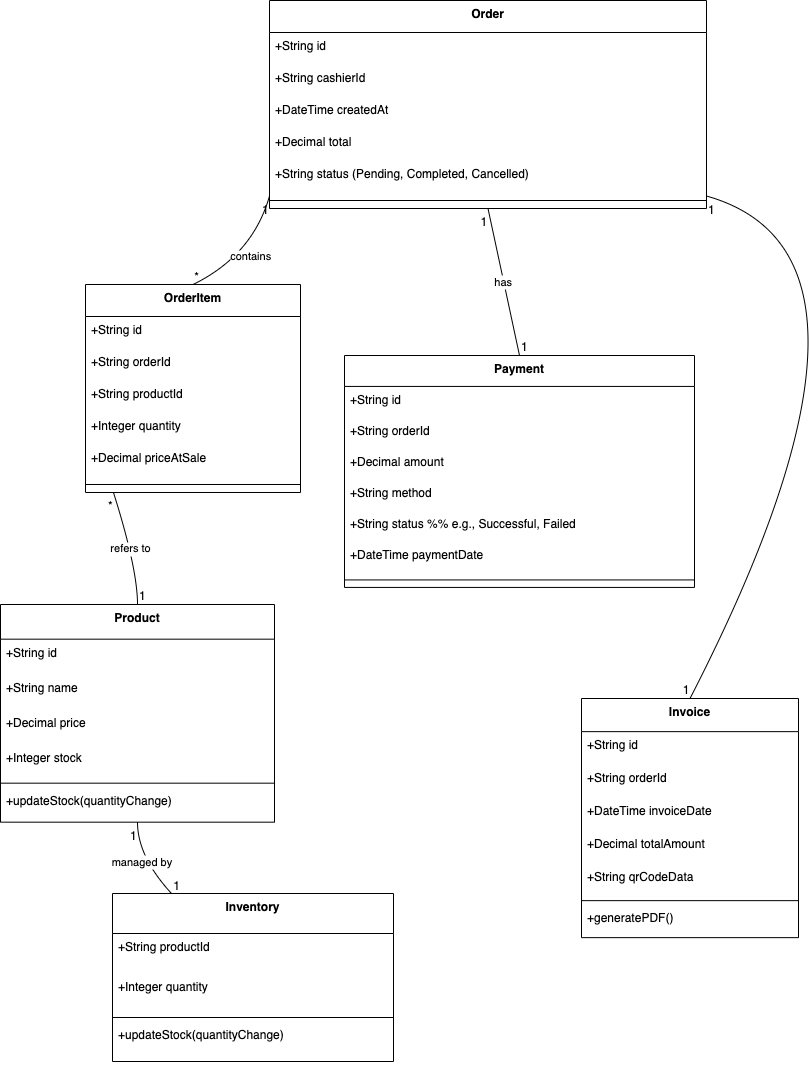
\includegraphics[width=0.9\textwidth]{figures/images/sprint3class.png}
  \caption{Sprint 3 – POS and Transaction Class Diagram}
  \label{fig:sprint3-class}
\end{figure}

\section{Sequence Diagram}

\begin{figure}[H]
  \centering
  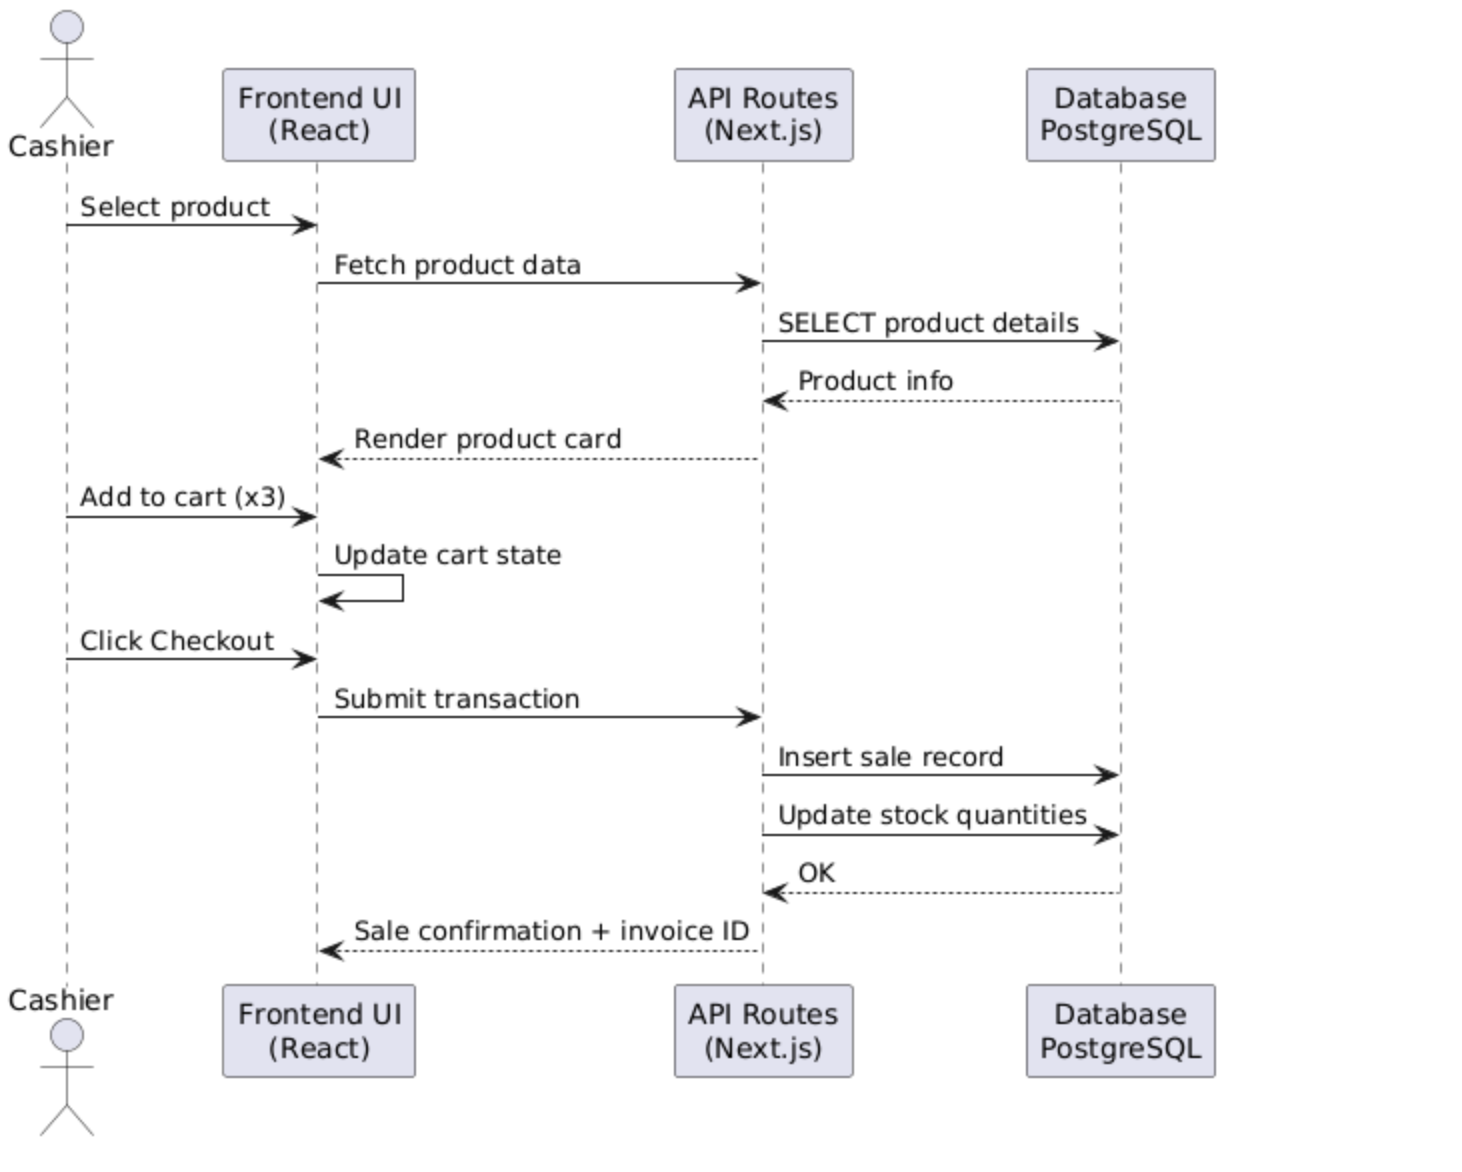
\includegraphics[width=0.9\textwidth]{figures/images/sprint3sequence.png}
  \caption{Sprint 3 – POS Transaction and Invoicing Sequence Diagram}
  \label{fig:sprint3-sequence}
\end{figure}

\section{API Architecture for POS Operations}

RESTful endpoints supporting the POS interface:

\subsection*{Product and Cart APIs}
\begin{itemize}
  \item \texttt{GET /api/pos/products} – Retrieve available products for sale
  \item \texttt{POST /api/pos/cart/add} – Add item to current session cart
  \item \texttt{PUT /api/pos/cart/update} – Modify cart item quantities
  \item \texttt{DELETE /api/pos/cart/remove} – Remove items from cart
\end{itemize}

\subsection*{Transaction APIs}
\begin{itemize}
  \item \texttt{POST /api/pos/checkout} – Process payment and create transaction
  \item \texttt{GET /api/pos/invoice/[id]} – Retrieve invoice details
  \item \texttt{GET /api/pos/transactions} – Access transaction history
\end{itemize}

\section{Security and Data Integrity}

\subsection*{Transaction Security}

Security measures implemented:
\begin{itemize}
  \item Session-based cart management to prevent data loss
  \item Transaction atomicity ensuring data consistency
  \item Payment processing validation and error handling
  \item Audit logging for all financial transactions
  \item User authentication verification for all operations
\end{itemize}

\subsection*{Data Validation}

Input validation includes:
\begin{itemize}
  \item Cart item quantity limits and stock availability
  \item Payment amount validation and calculation verification
  \item Product price consistency checking
  \item Transaction integrity validation
\end{itemize}

\section{Performance Optimization}

\subsection*{Frontend Performance}

Optimization techniques applied:
\begin{itemize}
  \item Product image lazy loading and caching
  \item Cart state management with local storage backup
  \item Debounced search and filtering functions
  \item Optimized re-renders using React memoization
\end{itemize}

\subsection*{Backend Performance}

Server-side optimizations:
\begin{itemize}
  \item Database indexing for fast product queries
  \item Connection pooling for concurrent transactions
  \item Cached product data for frequent access
  \item Efficient PDF generation with streaming
\end{itemize}

\section{Testing and Quality Assurance}

Comprehensive testing covered:

\begin{itemize}
  \item Product selection and cart management workflows
  \item Payment processing for all supported methods
  \item Invoice generation and PDF download functionality
  \item Stock deduction accuracy and inventory synchronization
  \item Error handling for network issues and validation failures
  \item User interface responsiveness across different devices
  \item Performance testing under simulated high transaction volumes
\end{itemize}

Manual testing validated all user workflows and edge cases, ensuring reliable operation under various conditions.

\section{Implementation Results}

The POS interface and invoicing system were successfully implemented, providing a complete solution for cashier operations.

% POS Interface Screenshots
\begin{figure}[H]
  \centering
  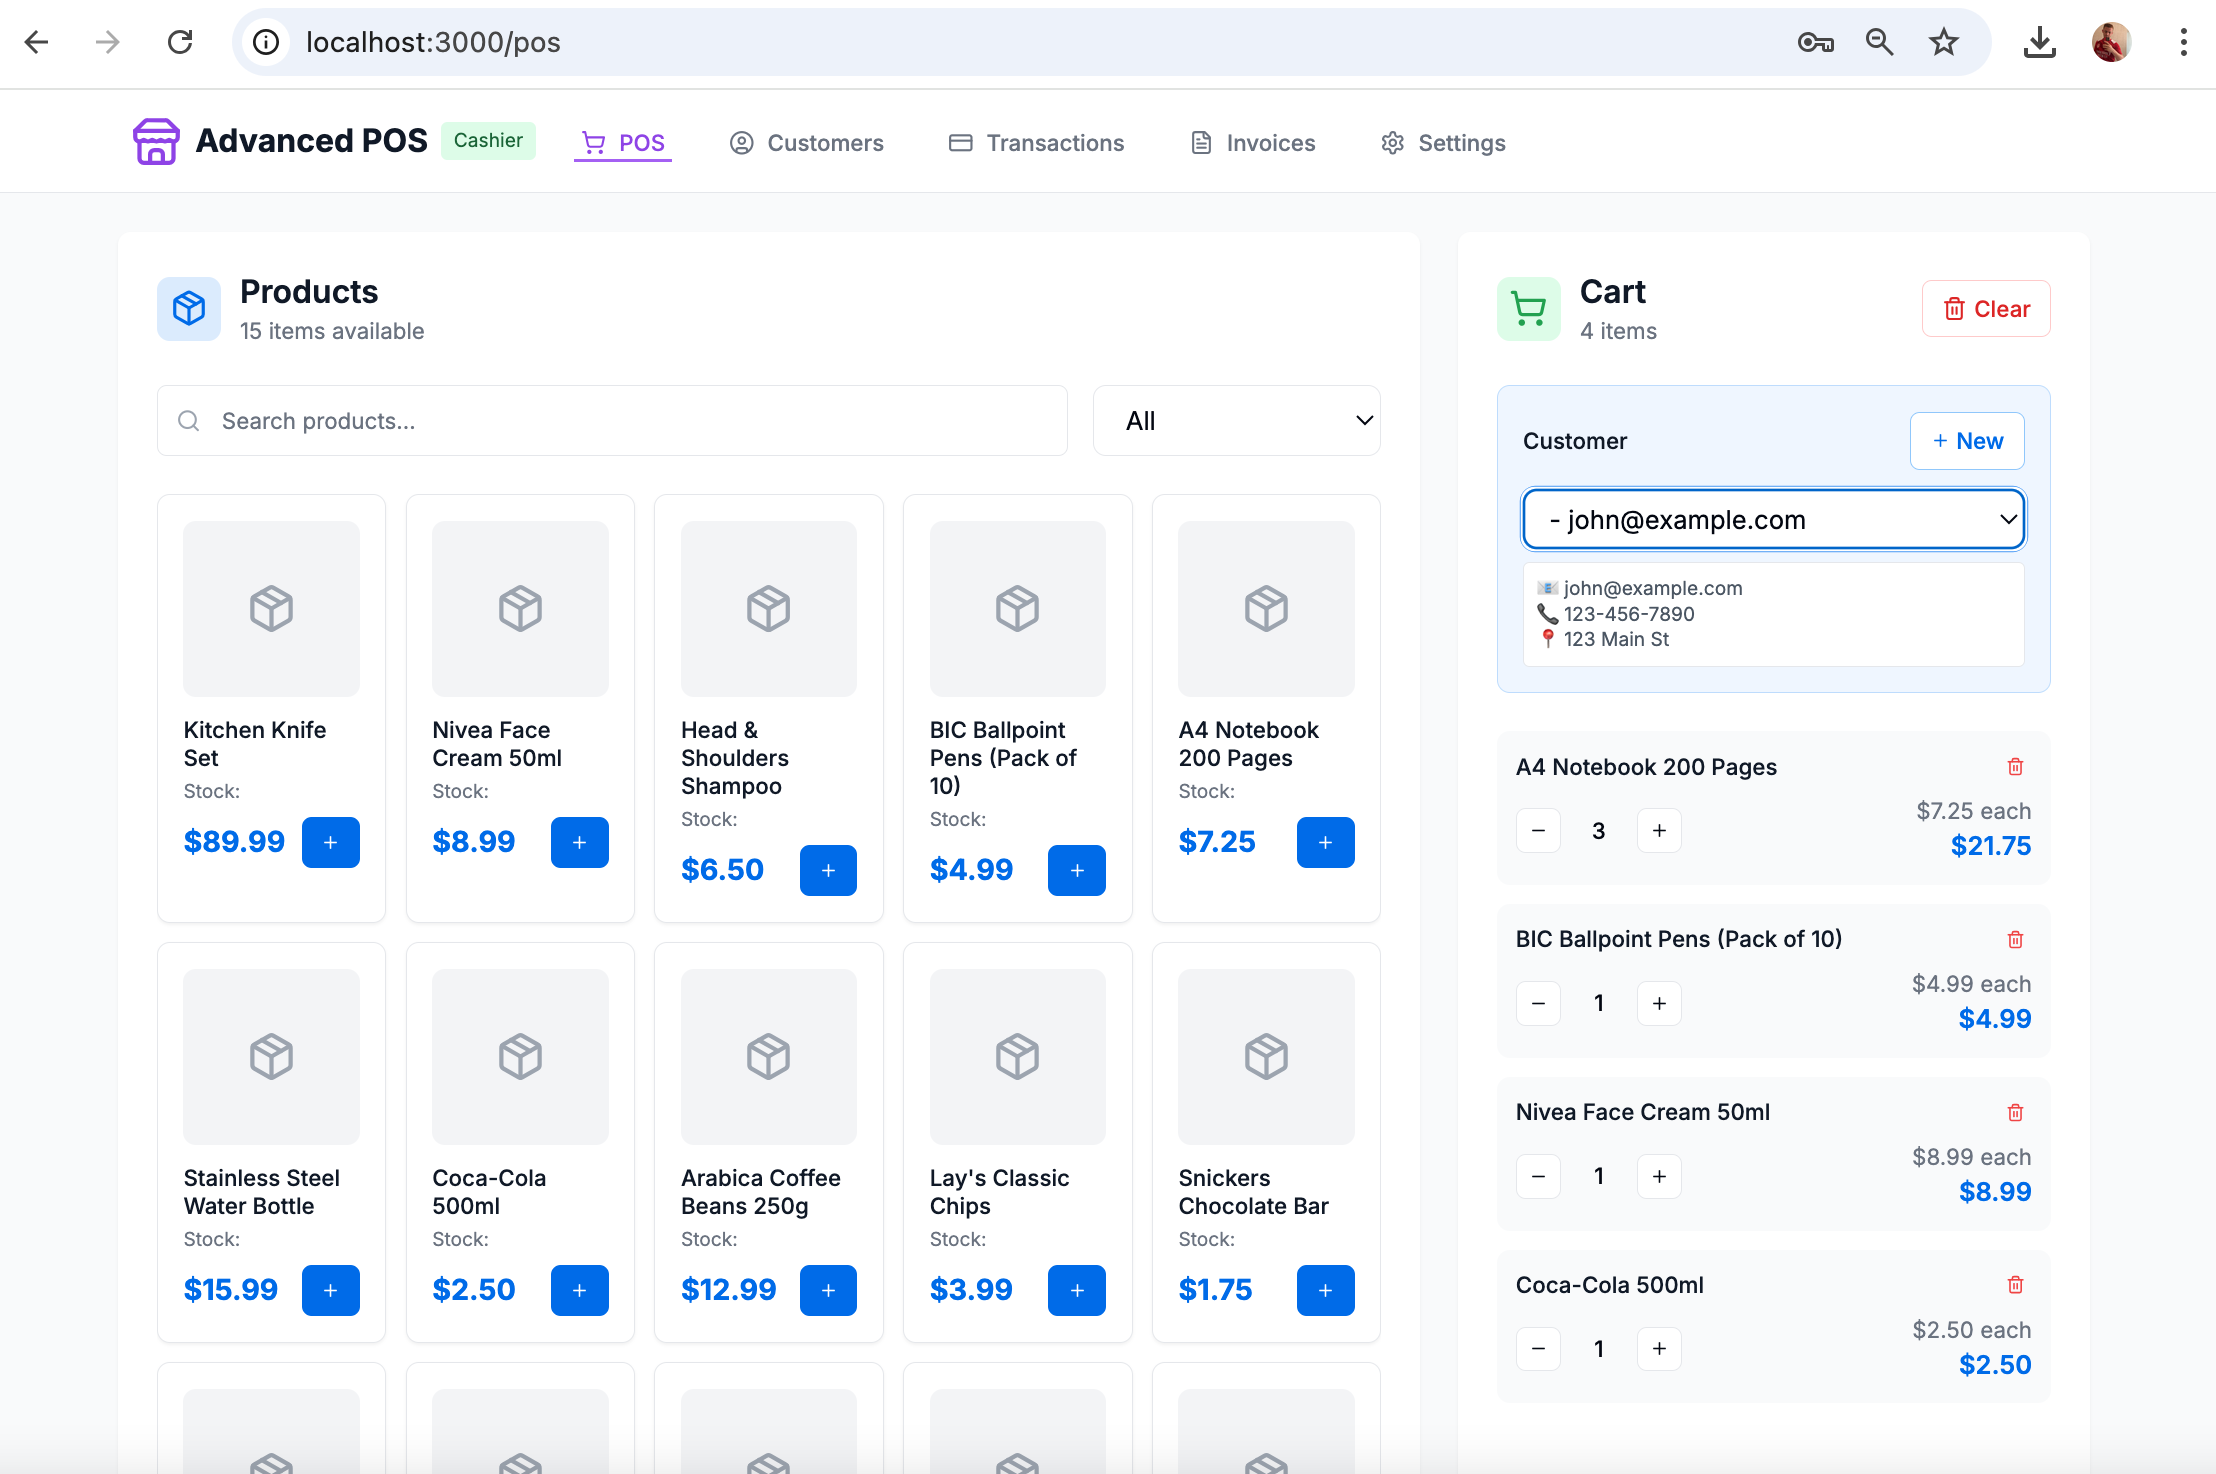
\includegraphics[width=0.9\textwidth]{working app screenshots/posinterface.png}
  \caption{POS Cashier Interface - Main point of sale dashboard with product grid and shopping cart}
  \label{fig:posinterface}
\end{figure}

\begin{figure}[H]
  \centering
  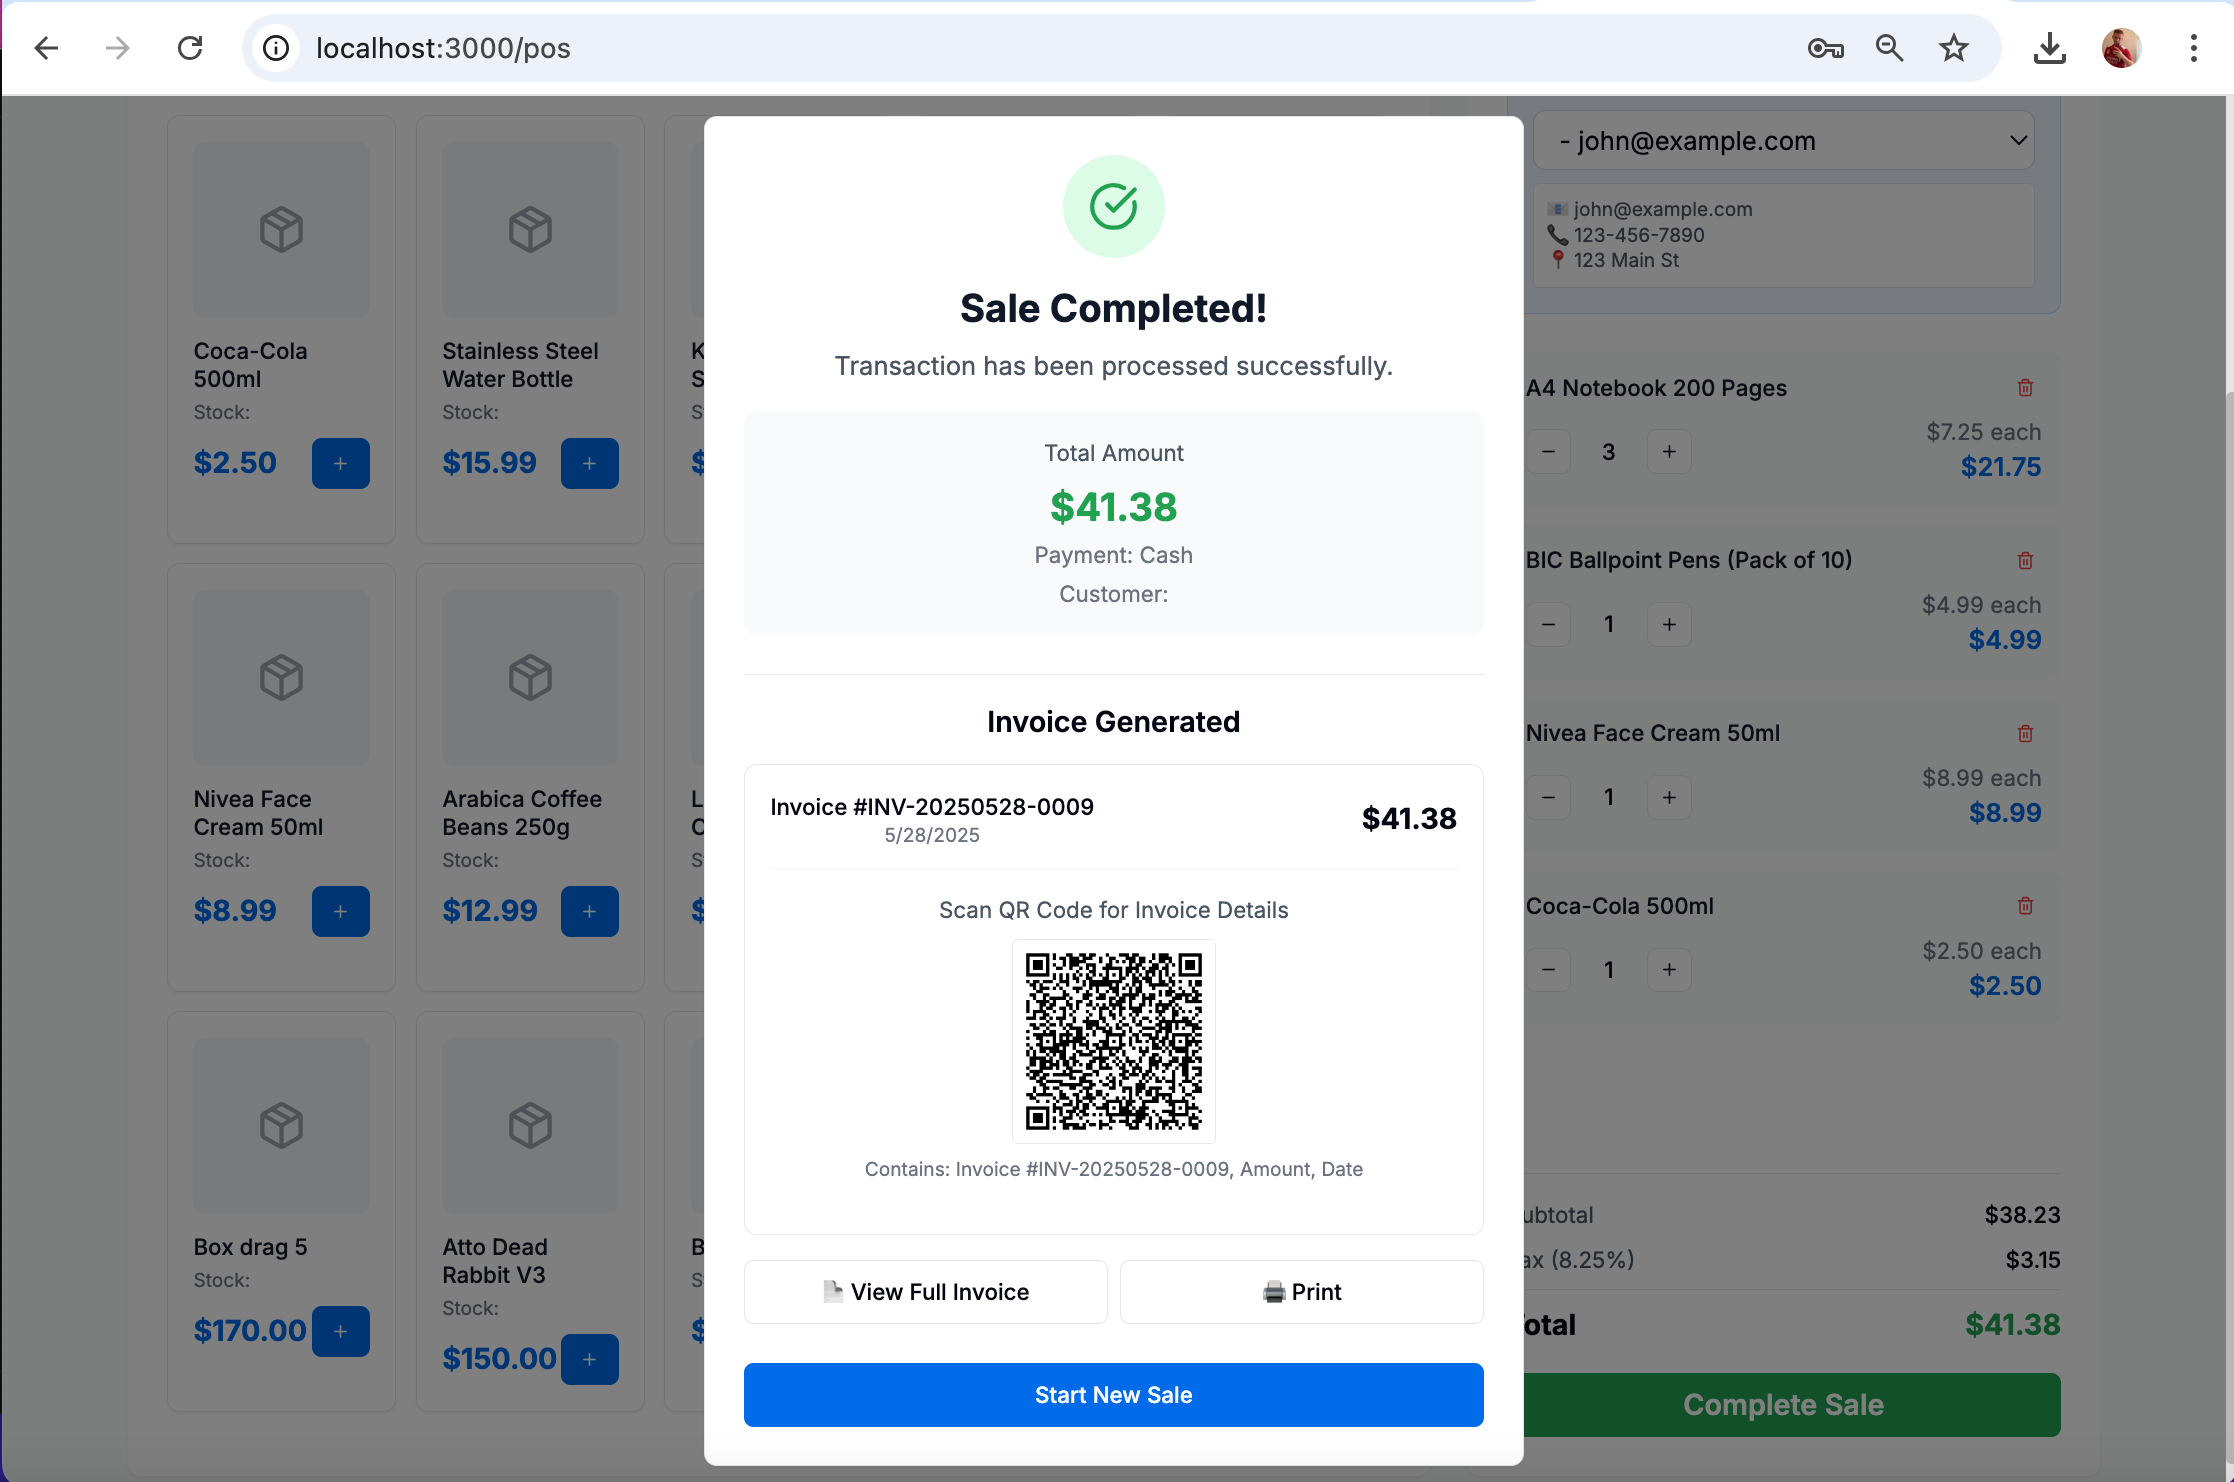
\includegraphics[width=0.9\textwidth]{working app screenshots/invoicegenerated.png}
  \caption{Generated Invoice - Professional invoice with transaction details and QR code}
  \label{fig:invoicegenerated}
\end{figure}

\begin{figure}[H]
  \centering
  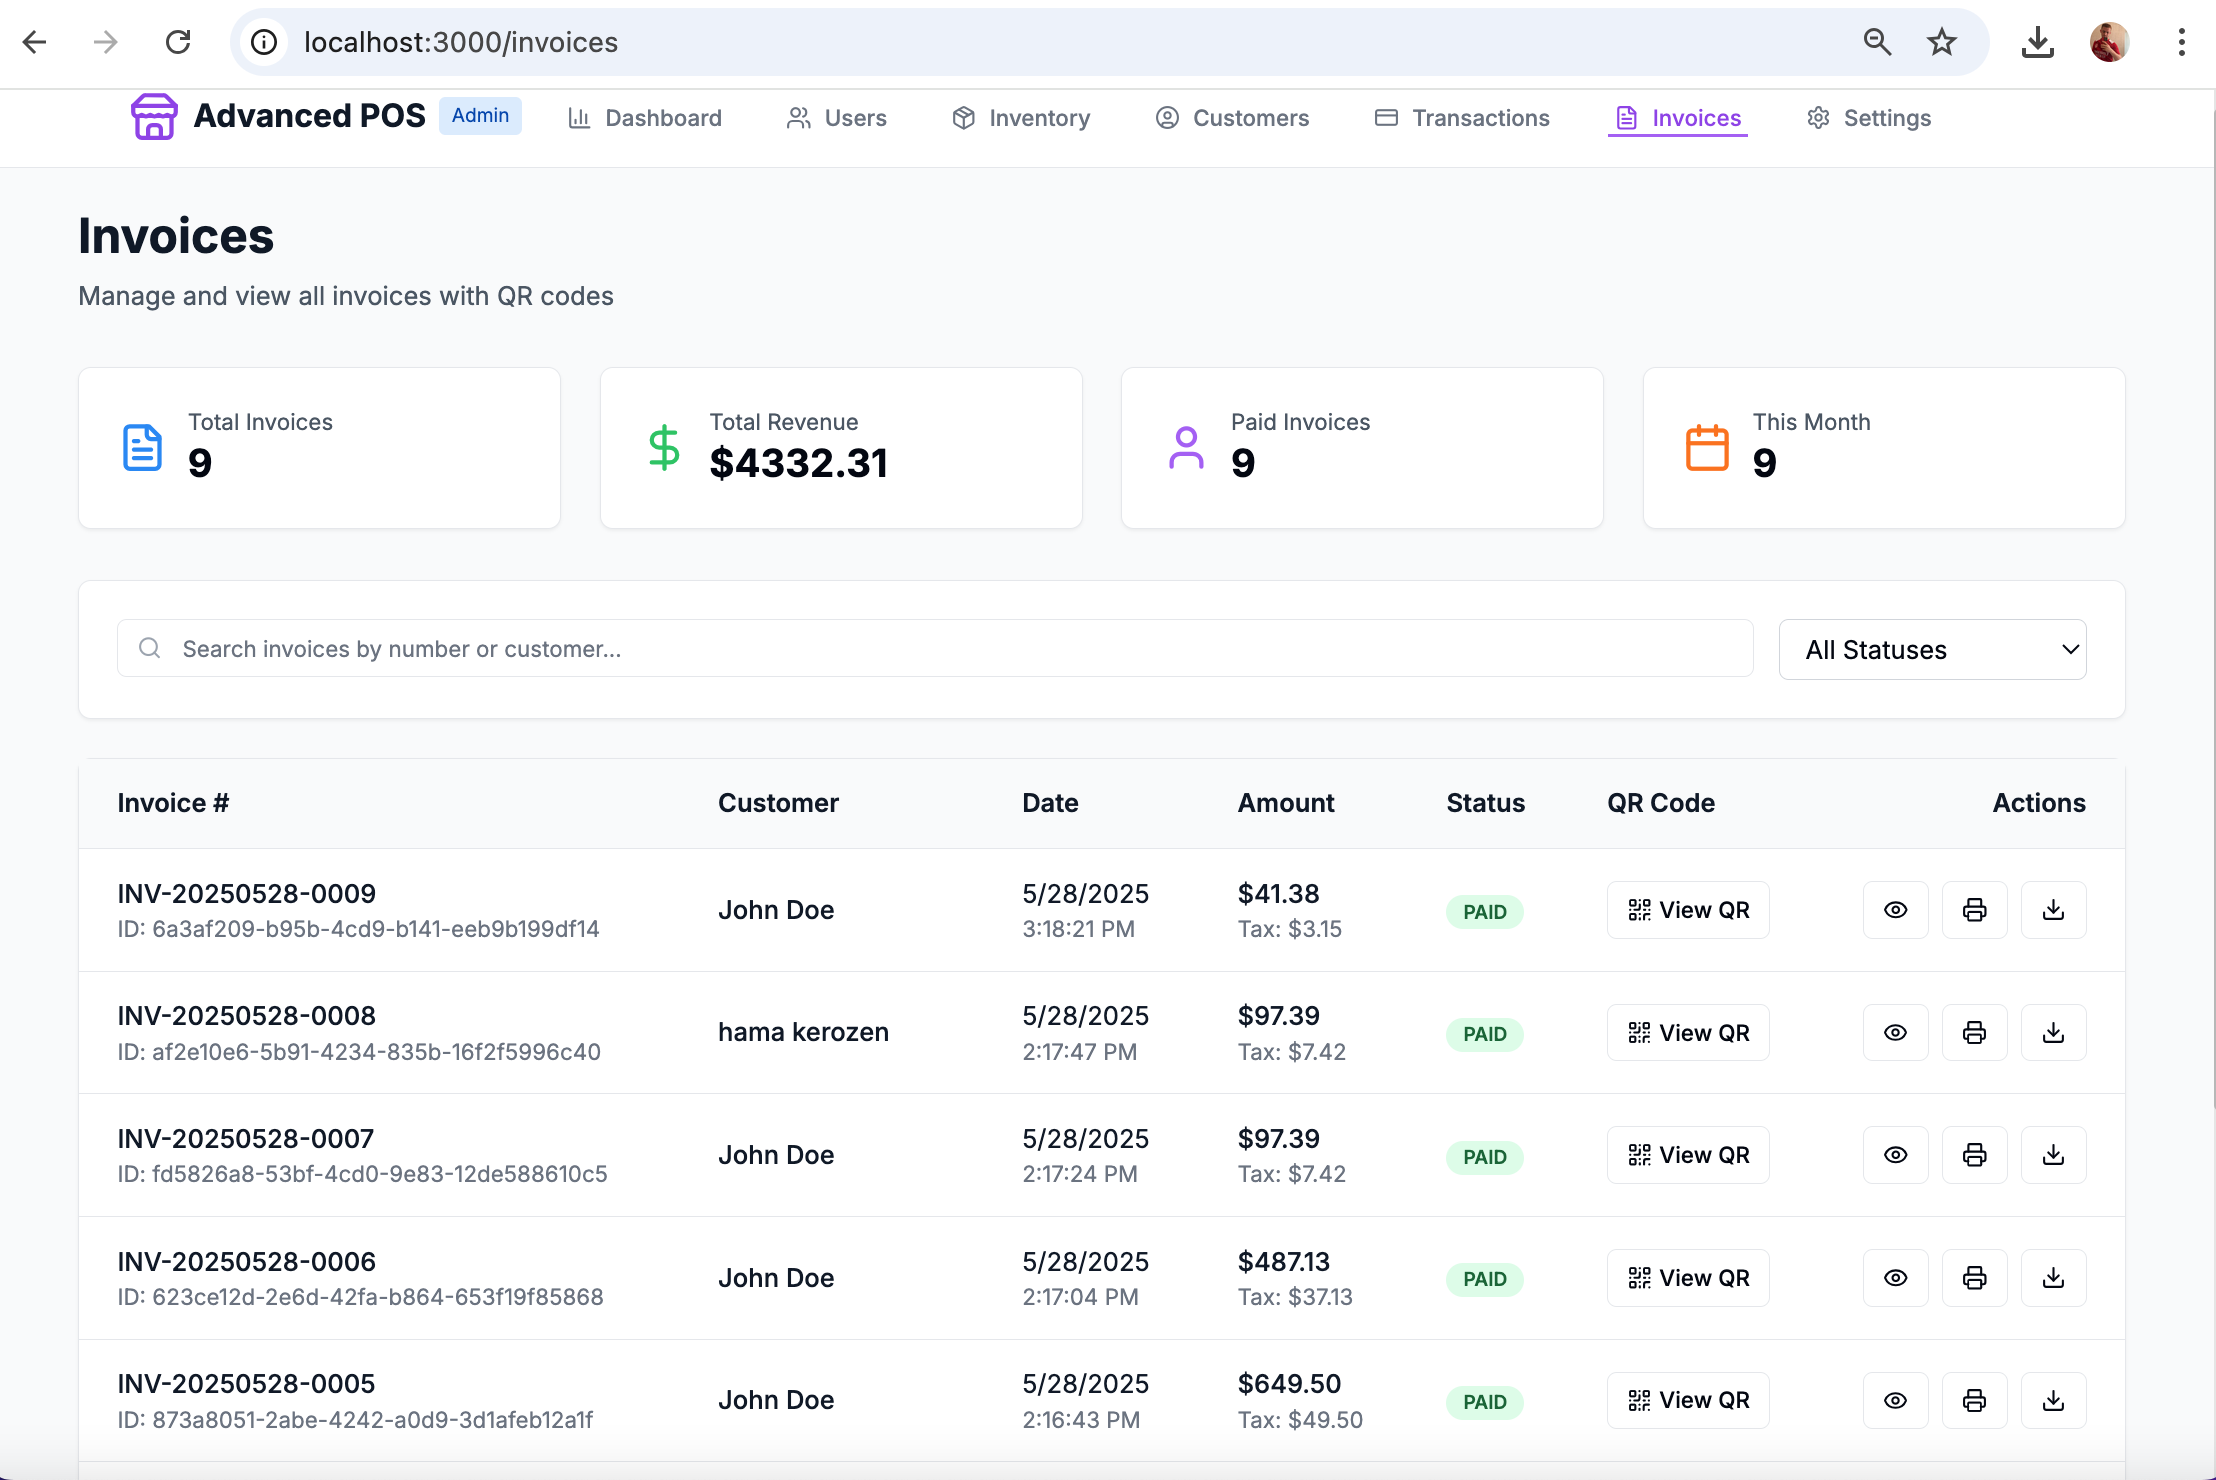
\includegraphics[width=0.9\textwidth]{working app screenshots/invoicedetails.png}
  \caption{Invoice Details View - Detailed breakdown of transaction items and pricing}
  \label{fig:invoicedetails}
\end{figure}

The POS system delivers:

\begin{itemize}
  \item Intuitive cashier interface with efficient product selection and cart management
  \item Seamless payment processing supporting multiple payment methods
  \item Professional invoice generation with automatic PDF creation and QR code embedding
  \item Real-time inventory updates ensuring accurate stock levels
  \item Comprehensive transaction logging for audit trails and reporting
  \item Responsive design optimized for touch-screen interactions and various device sizes
\end{itemize}

\section{Conclusion}

Sprint 3 successfully delivered a complete POS interface with comprehensive invoicing capabilities. Cashiers can now efficiently process sales through an intuitive interface while the system automatically handles invoice generation, stock updates, and transaction logging. The implementation provides a solid foundation for daily retail operations with professional invoice output and robust data management. The next sprint will focus on business intelligence integration and system finalization.
